\documentclass[12pt]{article}
\usepackage{graphicx, amsmath, amssymb, geometry, subcaption, hyperref} % Required for inserting images

\title{Y7 Starters}
\author{Ciaran Barnes}
\date{October 2023}

\geometry{margin=1in}
\pagenumbering{gobble}

\begin{document}

\maketitle
\tableofcontents
\begin{abstract}
    A collection of assorted Year 7 worksheets. The self-assessment tasks in Summer HT1 are particularly good revision ahead of summer assessments.
\end{abstract}

\newpage

\section{Retrieval/Mixed Practice}

\subsection{Autumn HT1}

\newpage

\subsection{Autumn HT2}

\begin{enumerate}
    \item Evaluate -17+9
    \item Evaluate \(-180 \div 12\)
    \item Simplify \(\sqrt{20}\)
    \item Simplify \( \sqrt{108} \)
    \item Evaluate \(-3 + 9 \div 6 \times 2^2  \)
    \item Evaluate \((7-12)^2 \times (3^3-17) \div 2\)
    \item Evaluate \( \sqrt[3]{729}\)
    \item Evaluate \(\sqrt{256}\)
    \item Find the prime factorisation of \(84\)
    \item Find the prime factorisation of \(612\)
\end{enumerate}

\newpage

\noindent \textbf{Starter}

\medskip

\hrule 

\medskip

\begin{enumerate}
    \item Sketch the line \(y=x\)
    \item Sketch the line \(x=-2\)
    \item Sketch the line \(y=-x\)
    \item Sketch the line \(y=3\)
    \item Does the point \((-1,1)\) lie on any of the above lines? If so, which line?
    \item Does the point \((-3,2)\) lie on any of the above lines? If so, which line?
    \item Simplify \(2(3+x)\)
    \item Simplify \(7(4-y)\)
    \item Simplify \(-3(z-1)\)
    \item Simplify \( x(12-x)\)
    \item Simplify \( -3y(1+y)\)
    \item Simplify \(-2z^2(3z-5)\)
    \item Simplify \(2x(x+1)+3(x-4)\)
    \item Simplify \( 3x(1-x) - 4x^2(1+2x) \)
    
\end{enumerate}

\newpage

\noindent \textbf{Starter}

\medskip

\hrule

\medskip

\begin{enumerate}
    \item Solve \(2x+1=7\)
    \item Solve \(9-2y=-4\)
    \item Solve \(\frac{5z+2}{-4}=5\)
    \item Evaluate \(1\frac{5}{12}+\frac{2}{3}\)
    \item Solve \(1-2(w-4)=5\)
    \item Evaluate \(7\frac{1}{5}-2\frac{5}{6}\)
    \item Evaluate \(\frac{196}{25} \times \frac{65}{28}\)
    \item Evaluate \(-2\frac{3}{5}\div 3\frac{3}{4}\)
\end{enumerate}

\newpage

\noindent \textbf{Answers}

\medskip

\hrule 

\medskip

\begin{enumerate}
    \item \(x=3\)
    \item \(y=6\frac{1}{2}\)
    \item \(z=-3\frac{3}{5}\)
    \item \(w=2\)
    \item \(2\frac{1}{12}\)
    \item \(4\frac{11}{30}\)
    \item \(18\frac{1}{5}\)
    \item \(-\frac{52}{75}\)
\end{enumerate}

\newpage

\noindent \textbf{Autumn Term Review Homework}

\medskip

\hrule

\medskip

\noindent Solve the following questions. The solution to each has a corresponding letter given on the page overleaf. Solve each question to reveal the hidden message.

\begin{enumerate}
    \item Evaluate \(17-23+4\)
    \item Evaluate \((3-5)^3\div 16 \times 7\)
    \item Evaluate \(0.738 \div 0.18\)
    \item Evaluate \(-3.94+8.04\)
    \item Simplify fully \(\sqrt{72}\)
    \item Determine \(0.0030721451\) accurate to 3 significant figures.
    \item Determine the index of 7 in the prime factorisation of 271656.
    \item Evaluate \(3.2 \times 1.28125\)
    \item Determine the coefficient of \(x^2\) in the expansion of \(7x(3-x)-x^2(x-1)\) 
    \item Evaluate \(-\frac{13}{9}+1\frac{1}{3}\)
    \item Substitute \(x=-2\) into the expression \(3x^2-7x\)
    \item Determine the \(x\)-coordinate of the intersection between the lines \(y=-x\) and \(y=2\)?
    \item An isosceles triangle has angles 54\(^\circ\) and 62\(^\circ\). What is the missing angle?
    \item Evaluate \(\frac{3}{16} \times \big(\frac{1}{3}-1 \big)^3 \div \frac{1}{2}\)
\end{enumerate}

\newpage

\noindent A \quad 62\\
B \quad 54 \\
C \quad 0.00307 \\
D \quad \(3\frac{1}{2}\)\\
E \quad \(-3\frac{1}{2}\)\\
F \quad \(4.231\)\\
G \quad 0.003\\
H \quad 3 \\
I \quad -6 \\
J \quad \(-1\frac{3}{7}\)\\
K \quad \(2\sqrt{18}\)\\
L \quad 8\\ 
M  \quad -2\\ 
N \quad 0.00\\
N \quad \(3\sqrt{8}\)\\
O \quad -8\\
P \quad 0.003072\\
Q \quad -26\\
R \quad 4.1\\
S \quad \(-\frac{1}{9}\)\\
T \quad 26 \\
U \quad \(\pi\)\\
V \quad \(6\sqrt{3}\)\\
W \quad 6\\
X \quad 2\\
Y \quad \(6\sqrt{2}\)\\
Z \quad \(\frac{7}{12}\)\\


\newpage

\subsection{Spring HT2}

\newpage

\noindent \textbf{Retrieval Practice}

\medskip

\hrule

\medskip

\begin{enumerate}
    \item Evaluate \(2+12^2\div6 \)
    \item Determine the prime factorisation of 1386.
    \item Sketch a graph of \(y=4\) and \(y=-x\). At which coordinate do they intersect?
    \item Determine \(\frac{7}{5}-1\frac{2}{15}\)
    \item In the graph below, fully describe two transformations from \(A\) to \(B\).
\end{enumerate}

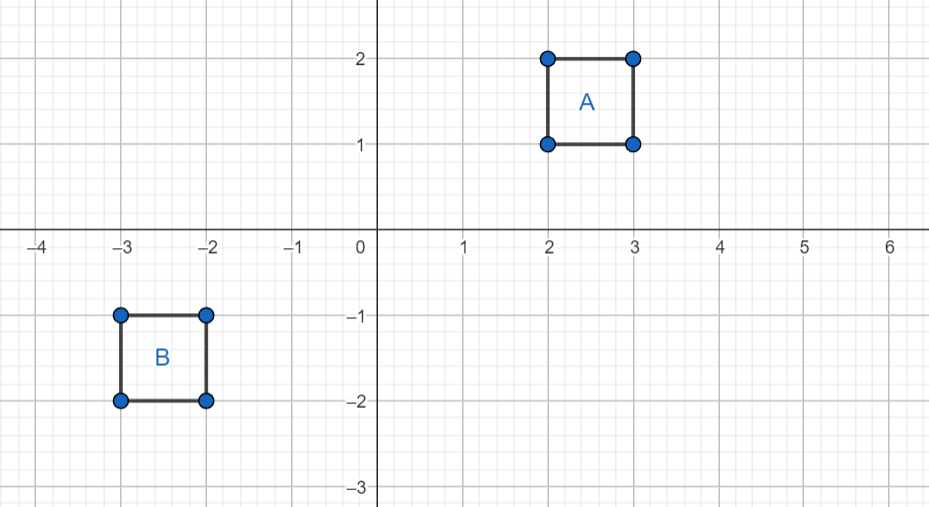
\includegraphics[]{0 - Retrieval Revision/Retrieval2.PNG}

\newpage

\subsection{Summer HT1}

\newpage

\noindent \textbf{Self-Assessment Task 1}

\medskip

\hrule

\medskip

\begin{enumerate}
    \item Solve \(3x-7=59\).
    \item Evaluate \(15-6^2\div3\).
    \item Plot the line \(y=-3\) in Figure 1 below.
    \item Evaluate \((-3)^3 \div \big( -2+(-4)\big)\) as an improper fraction.
    \item Solve \(5x-20 = 4-3x\).
    \item Plot the coordinates \((-1,2), (3,4)\) and \((5,0)\) on Figure 1 below.
    \item What coordinate is now needed to form a rectangle in Figure 1?
    \item Solve \(\frac{4}{9}x - 2 = \frac{1}{3}(x+1)\).
    \item Evaluate \(16 \div 8 \div (4 \div 2)\).
    \item Evaluate \(\frac{1}{1+\frac{1}{1+\frac{1}{3+\frac{1}{4}}}}\).
\end{enumerate}

\begin{figure}[ht]
    \centering
    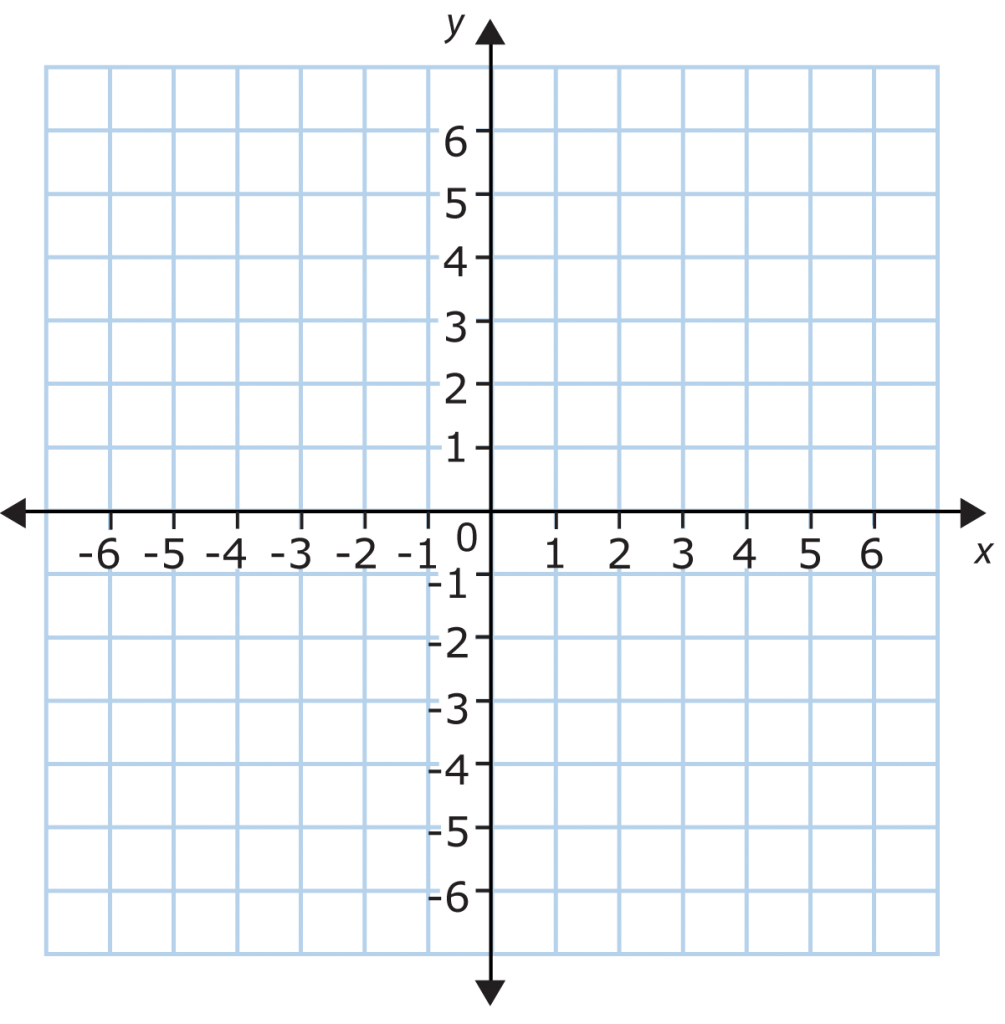
\includegraphics[width=0.5\textwidth]{image3.png}
    \caption{}
    \label{fig:enter-label}
\end{figure}

\newpage

\noindent \textbf{Self-Assessment Task 2}

\medskip

\hrule

\medskip

\begin{enumerate}
    \item Evaluate \(0.00321 \times 0.014\).
    \item Translate shape \(A\) in Fig. (a) by the vector \(\begin{pmatrix}
        4 \\
        3
    \end{pmatrix}\).
    \item Evaluate \(\frac{17}{19}+ \frac{12}{57}\) as a mixed number.
    \item Reflect shape \(A\) in Fig. (a) about the line \(y=x\).
    \item Evaluate \(2.25 \div 0.0045\).
    \item Describe fully the transformation from \(A\) to \(B\) shown in Fig. (b).
    \item Evaluate \(\frac{125}{27}\div1\frac{2}{3}\) as a mixed number.
    \item State 0.021004 to 3 significant figures.
    \item Evaluate \(-\frac{5}{9}+\big(-\frac{4}{5}\big)^2\).
    \item A number after being rounded to 2 significant figures is 100. What is the lowest value this number could be?
\end{enumerate}



\begin{figure}[ht]

\begin{subfigure}{0.5\textwidth}
    \centering
    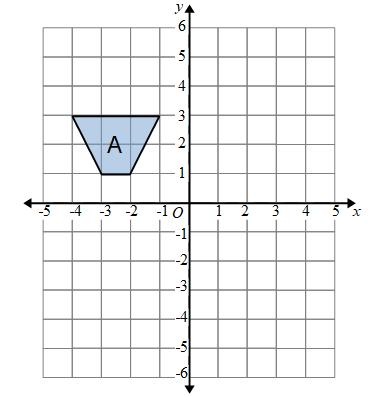
\includegraphics[width=0.9\linewidth]{image2.png}
    \caption{}
\end{subfigure}
\begin{subfigure}{0.5\textwidth}
    \centering
    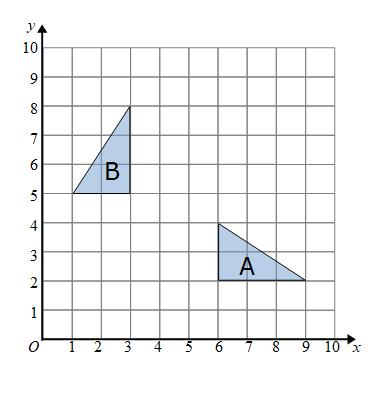
\includegraphics[width=0.9\linewidth]{image1.png}
    \caption{}
\end{subfigure}
    
\end{figure}


\newpage

\noindent \textbf{Self-Assessment Task 3}

\medskip

\hrule

\medskip

\begin{enumerate}
    \item Simplify the following expression \(3x(x-4) + 5x\).
    \item A triangle has side lengths of 2cm, 4cm and 6cm. Is this a right angled triangle? Explain your answer fully.
    \item In the triangle shown below in figure (a), \(AB=2.4\)cm and \(BC=2.5\)cm. Determine the length of \(AC\).
    \item Determine the size of angle \(x\) in figure (b) below.
    \item Substitute \(a=2\) and \(b=-0.5\) into the expression \(\frac{a+b^2}{2ab}\).
    \item Determine the size of angle \(y\) in figure (b) below.
    \item Simplify the following expression \(2xy^2 - 2xy + 2 x^2y - 2xy + 2xy^2\).
    \item Determine the size of angle \(y\) in figure (c). Give reasons for your answer.
    \item Determine the distance between the points \((3, -2)\) and \((-2, -14)\).
    \item Determine the length \(DE\) in figure (d) if the total area of \(ABCED\) is 60 cm\(^2\).
\end{enumerate}

\begin{figure}[ht]

\begin{subfigure}{0.5\textwidth}
    \centering
    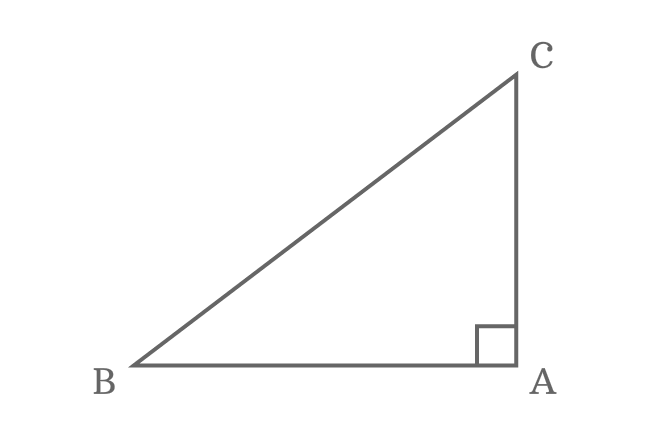
\includegraphics[width=0.7 \linewidth]{image4.png}
    \caption{}
\end{subfigure}
\begin{subfigure}{0.5\textwidth}
    \centering
    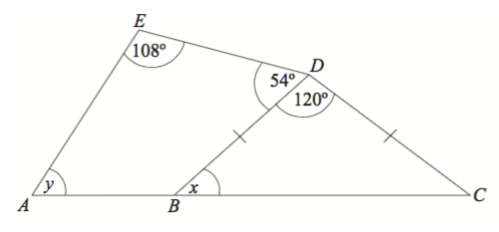
\includegraphics[width=\linewidth]{image5.png}
    \caption{}
\end{subfigure}

\begin{subfigure}{0.5\textwidth}
    \centering
    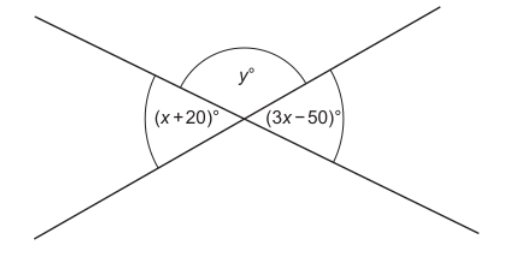
\includegraphics[width=0.9\linewidth]{image6.png}
    \caption{}
\end{subfigure}
\begin{subfigure}{0.5\textwidth}
    \centering
    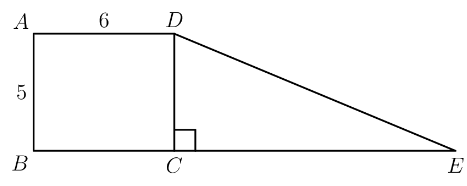
\includegraphics[width=0.9\linewidth]{image7.png}
    \caption{}
\end{subfigure}

\end{figure}

\newpage

\noindent \textbf{Self-Assessment Task 4}

\medskip

\hrule

\medskip

\begin{enumerate}
    \item Determine the probability of obtaining two heads when a coin is flipped three times.
    \item Plot the line \(y=2x-2\) on graph (a) below.
    \item Having plotted \(y=2x-2\), state the equation of the line that would need to be plotted to graphically solve the equation \(-3x+4=2x-2\)
    \item Convert 3.3125 into a fraction.
    \item If a biased dice has a probability of 0.4 of landing on a 6, what is the expected number of sixes in 250 rolls?
    \item Find 17.5\% of 24.
    \item A four sided spinner can land on any colour of: blue, red, green and yellow. The probability of landing on red is 0.2 and on blue is 0.35. The probability of landing on yellow is 14 times smaller than that of green. Determine the probability of landing on green.
    \item Use graph (b) to convert 10 miles into km.
    \item Evaluate \(16.2\% - \frac{5}{8} \times 0.42\) 
    \item In a bag there are 4 blue balls and \(x\) red balls. Adding 10 blue balls triples the probability of picking a blue. How many red balls are there?
\end{enumerate}

\begin{figure}[ht]

\begin{subfigure}{0.5\textwidth}
    \centering
    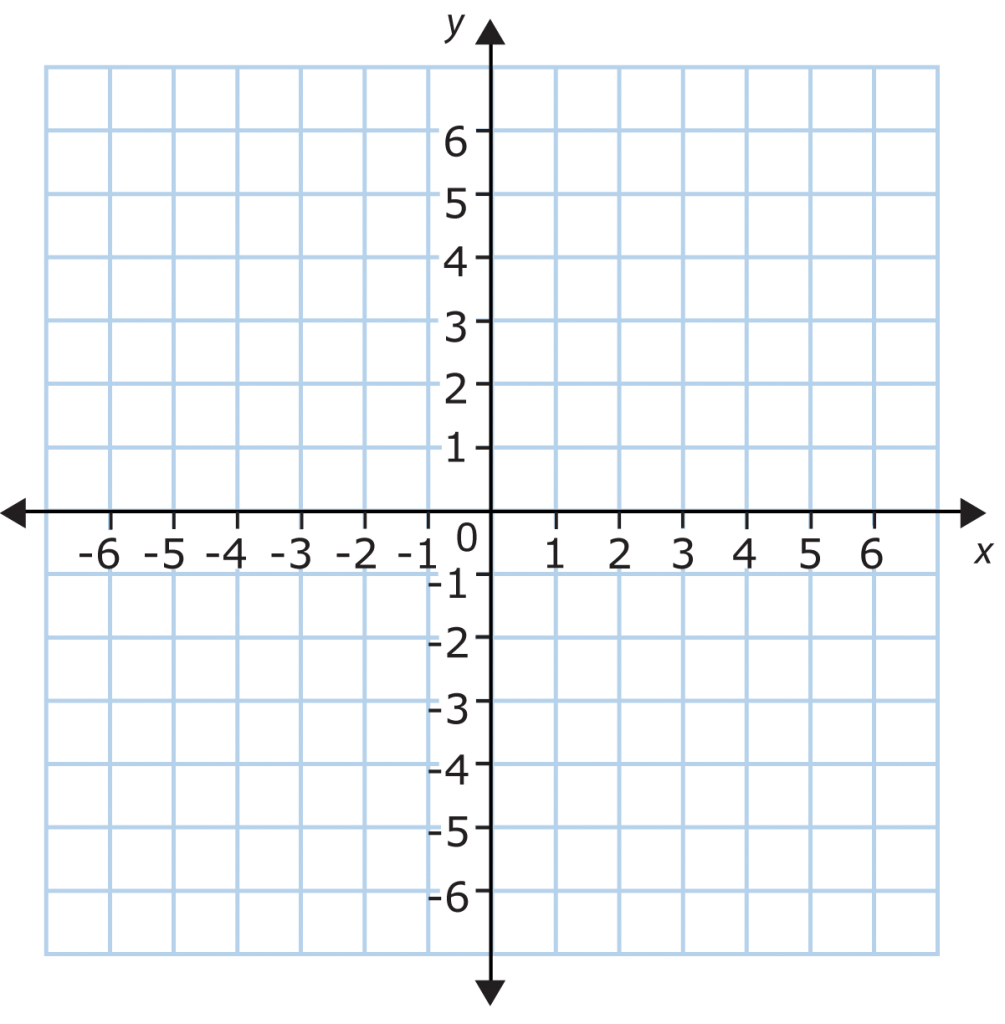
\includegraphics[width=0.9\linewidth]{image3.png}
    \caption{}
\end{subfigure}
\begin{subfigure}{0.5\textwidth}
    \centering
    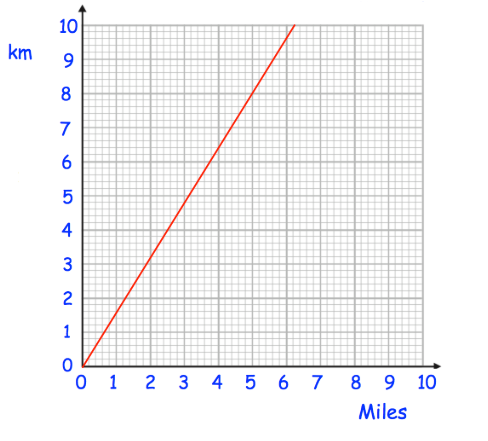
\includegraphics[width=\linewidth]{image8.png}
    \caption{}
\end{subfigure}

\end{figure}

\newpage

\noindent \textbf{Self-Assessment Task 5}

\medskip

\hrule

\medskip

\begin{enumerate}
    \item Determine the prime factorisation of 630.
    \item Lines \(ABC\) and \(DEF\) are parallel in figure (a). Determine the size of angle \(BEF\) stating a reason for your answer.
    \item Determine the prime factorisation of 13013.
    \item Determine a formula for the \(n^\text{th}\) term of the sequence given by \(3, \, -\frac{5}{2}, \, -8, \, -\frac{27}{2}, \, \dots\)
    \item Is 51 in the sequence defined by \(u_n = 7+3n\). Justify your answer.
    \item Determine, using prime factorisation, the square root of 5929.
    \item A sequence is defined by \(u_n=\frac{2n+1}{3-n}\). Determine the 5\(^\text{th}\) term in the sequence.
    \item In figure (b) below, you are given that the lines \(AB, \, CD,\) and \(EF\) are parallel. Determine the size of angle \(CFE\).
    \item In figure (c), \(AFE\) and \(BCD\) are straight lines. Prove that they are parallel.
    \item Determine whether or not 41075800 is a cube or not. Justify your answer.
    %\medskip \\
    %\textbf{Hint:} you do not need to do a full prime factorisation.
\end{enumerate}

\begin{figure}[ht]
    \begin{subfigure}{0.5\textwidth}
        \centering
        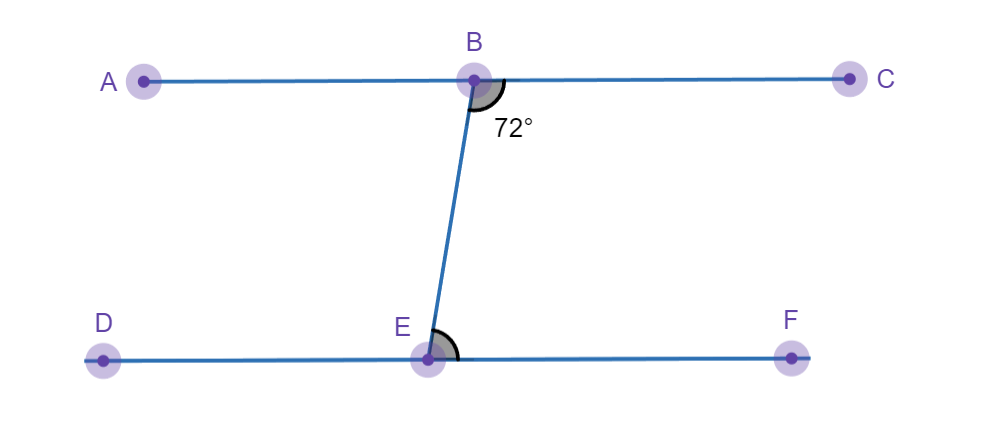
\includegraphics[width=\linewidth]{image9.png}
        \caption{}
    \end{subfigure}
    \begin{subfigure}{0.5\textwidth}
        \centering
        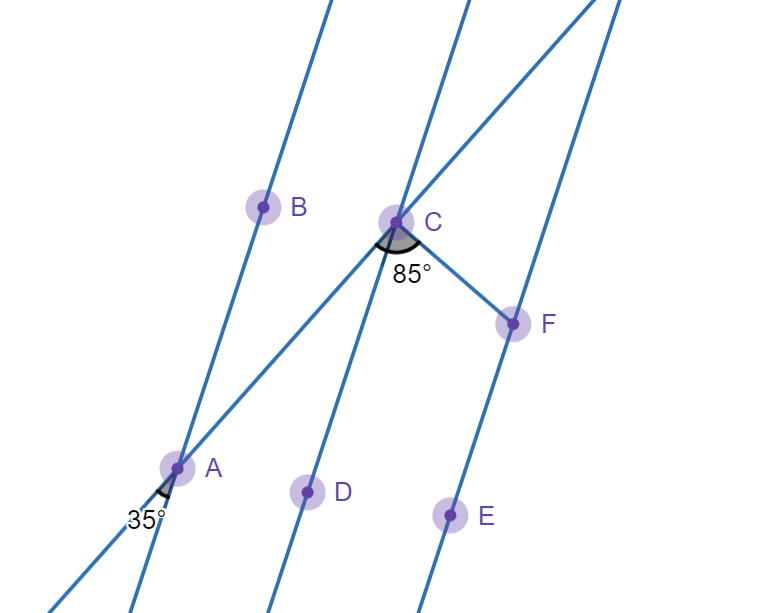
\includegraphics[width=0.9\linewidth]{image10.png}
        \caption{}
    \end{subfigure}
    
    \begin{subfigure}{0.5\textwidth}
        \centering
        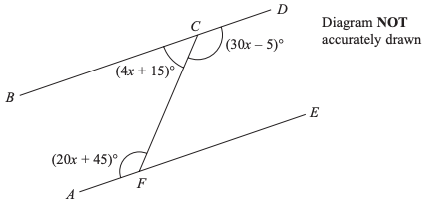
\includegraphics[width=\linewidth]{image11.png}
        \caption{}
        
    \end{subfigure}
\end{figure}

\newpage

\section{Fractions}

\newpage

\noindent \textbf{Fraction Arithmetic}

\medskip

\hrule 

\medskip

\noindent Give all answers as mixed numbers where appropriate.

\begin{enumerate}
    \item \(\frac{2}{7}+ \frac{3}{5}\)
    \item \(\frac{3}{4} - \frac{1}{6}\)
    \item \(\frac{2}{5} \times \frac{9}{11}\)
    \item \(\frac{13}{19} \times \frac{3}{26}\)
    \item \( \frac{7}{8} \div \frac{1}{4} \)
    \item \( 3\frac{1}{4} + 2\frac{4}{5} \)
    \item \(5\frac{5}{12} - 3\frac{2}{3}\)
    \item \(2\frac{2}{15} \times 1\frac{1}{4}\)
    \item \(3\frac{2}{3} \div 1\frac{2}{5}\)
    \item \(\big(\frac{6}{7}\big)^3\)
    
\end{enumerate}

\newpage

\noindent \textbf{Fraction Arithmetic} \hfill Answers

\medskip

\hrule 

\medskip

\begin{enumerate}
    \item \( \frac{31}{35} \)
    \item \( \frac{7}{12} \)
    \item \( \frac{18}{55} \)
    \item \( \frac{3}{38} \)
    \item \( 3\frac{1}{2} \)
    \item \( 6\frac{1}{20} \)
    \item \( 1 \frac{3}{4}\)
    \item \( 2\frac{2}{3} \)
    \item \( 2\frac{13}{21} \)
    \item \( \frac{216}{343} \)
\end{enumerate}

\section{Equations}

\newpage

\noindent \textbf{Solving Equations with Fractions Starter}

\medskip

\hrule 

\medskip

\noindent Solve the following equations:

\begin{enumerate}
    \item \( a + \frac{1}{2} = 3\)
    \item \(b - \frac{3}{5} = - \frac{1}{4}\)
    \item \( \frac{2}{3} c = 7 \)
    \item \( \frac{d}{7} = \frac{4}{11} \)
    \item \( \frac{3w}{-4} = \frac{9}{16} \)
    \item \( \frac{2}{5}x+1 =\frac{1}{3} \)
    \item \( \frac{3y}{7}-\frac{1}{4} = -2\)
    \item \( \frac{-2}{9}z-\frac{2}{3} = \frac{5}{9}\)
\end{enumerate}

\newpage

\noindent \textbf{Answers}

\medskip

\hrule 

\medskip

\begin{enumerate}
    \item \(a=2\frac{1}{2}\)
    \item \(b=\frac{7}{20}\)
    \item \(c=10\frac{1}{2}\)
    \item \(d=2\frac{6}{11}\)
    \item \(w=-\frac{3}{4}\)
    \item \(x = -1\frac{2}{3}\)
    \item \(y=-4\frac{1}{12}\)
    \item \(z=-5\frac{1}{2}\)
\end{enumerate}

\newpage

\noindent \textbf{Decimal Arithmetic and Solving Equations Starter}

\medskip

\hrule

\medskip

\begin{enumerate}
    \item Evaluate the following:
    \begin{enumerate}
        \item \(0.231 + 0.0416\)
        \item \(0.0415 - 0.278\)
        \item \(0.245 \times 3.1\)
        \item \(7.29 \div 0.081\)
    \end{enumerate}
    \item Solve the following equations for \(x\):
    \begin{enumerate}
        \item \(3x-4=-16\)
        \item \(3(x-2)-4(2x+5)=1\)
        \item \(-4x+2 = 7x -15\)
        \item \( \frac{2}{3}x-\frac{5}{6} = 5 \)
    \end{enumerate}
    \item Two lengths of an equilateral triangle are \(3x-1\) and \(x+2\). Form and solve an equation in \(x\).
\end{enumerate}

\newpage

\noindent \textbf{Decimal Arithmetic and Solving Equations Starter} \hfill Answers

\medskip

\hrule 

\medskip

\begin{enumerate}
    \item \begin{enumerate}
        \item 0.2726
        \item -0.2365
        \item 0.7595
        \item 90
    \end{enumerate}
    \item \begin{enumerate}
        \item \(x=-4\)
        \item \(x=-5\frac{2}{5}\)
        \item \(1\frac{6}{11}\)
        \item \(x=8\frac{3}{4}\)
    \end{enumerate}
    \item \(x=1\frac{1}{2}\)
\end{enumerate}

\newpage

\noindent \textbf{Fractions, Decimals and Percentages}

\medskip

\hrule 

\medskip

\begin{enumerate}
    \item Convert 0.825 into a fraction.
    \item Convert 32.5\% into a fraction in its simplest form.
    \item Write 3.015 as a percentage.
    \item Write \(\frac{17}{25}\) as a decimal.
    \item Find 93\% of 320.
    \item Find \(\frac{3}{5}\) of 72. Give your answer as a decimal.
    \item Increase 52 by 4\%.
    \item Decrease 36 by 12\%.
    \item If \(\frac{3}{17}\) of a quantity is 33, find the original quantity.
    \item Evaluate 0.23 - 16.5\% +\(\frac{5}{8}\) as a fraction.
\end{enumerate}

\newpage

\noindent \textbf{Fractions, Decimals and Percentages} \hfill Answers

\medskip

\hrule 

\medskip

\begin{enumerate}
    \item \(\frac{33}{40}\)
    \item \(\frac{13}{40}\)
    \item 301.5\%
    \item 0.68
    \item 297.6
    \item 43.2
    \item 54.08
    \item 31.68
    \item 187
    \item \(\frac{69}{100}\)
\end{enumerate}

\newpage

\section{BIDMAS, Powers, Surds and Negatives}

\newpage

\noindent \textbf{Surds}

\medskip

\hrule 

\medskip

\noindent Simplify the following surds:

\begin{enumerate}
    \item \(\sqrt{36}\)
    \item \(\sqrt{169}\)
    \item \(\sqrt{8}\)
    \item \(\sqrt{20}\)
    \item \(\sqrt{48}\)
    \item \(\sqrt{\frac{16}{25}}\)
    \item \(\sqrt{\frac{169}{144}}\)
    \item \(\sqrt{1\frac{34}{81}}\)
    \item \(\sqrt{6.25}\)
    \item \(\sqrt{0.5625}\)
\end{enumerate}

\newpage

\noindent \textbf{Surds} \hfill Answers

\medskip

\hrule 

\medskip

\begin{enumerate}
    \item 6
    \item \(13\)
    \item \(2\sqrt{2}\)
    \item \(2\sqrt{5}\)
    \item \(4\sqrt{3}\)
    \item \(\frac{4}{5}\)
    \item \(\frac{13}{12}\)
    \item \(1\frac{5}{9}\)
    \item \(\frac{5}{2}\)
    \item \(\frac{3}{4}\)
\end{enumerate}

\newpage

\noindent \textbf{Surds}

\medskip

\hrule 

\medskip

\noindent Simplify the following expressions:

\begin{enumerate}
    \item \(\sqrt{49}\)
    \item \(\sqrt{196}\)
    \item \(\sqrt{12}\)
    \item \(\sqrt{45}\)
    \item \(\sqrt{96}\)
    \item \(\sqrt{\frac{9}{64}}\)
    \item \(\sqrt{\frac{121}{324}}\)
    \item \(\sqrt{\frac{7}{144}}\)
    \item \(\big(\sqrt{10}\big)^2\)
    \item \(\big(3\sqrt{7}\big)^2\)
\end{enumerate}

\newpage

\section{Pythagoras}

\newpage

\noindent \textbf{Pythagoras Applications}

\medskip

\hrule 

\medskip

\begin{enumerate}
    \item Determine the distance between the following points. Give your answer as a simplified surd if necessary.
    \begin{enumerate}
        \item \((3,2)\) and \( (9, 10) \)
        \item \( (3,-13)\) and \( (-5, 2) \)
        \item \((5,2)\) and \((1,4)\)
        \item \((-1,-7)\) and \((5,-11)\)
    \end{enumerate}
    \item Determine two possible areas of an isosceles triangle with side lengths 3cm and 2cm.
    \item A parallelogram has an area of 12cm\(^2\) and on of the lengths is 8cm. Determine the remaining length.
\end{enumerate}

\newpage

\noindent \textbf{Pythagoras Applications} \hfill Answers

\medskip

\hrule 

\medskip

\begin{enumerate}
    \item \begin{enumerate}
        \item 10cm
        \item 17cm
        \item \(2\sqrt{5}\) cm
        \item \(2\sqrt{13}\) cm
    \end{enumerate}
    \item \(\frac{3\sqrt{13}}{8}\) or \(\sqrt{2}\)
    \item 
\end{enumerate}

\newpage

\section{Straight Line Graphs}

\newpage

\noindent \textbf{Plotting Straight Lines} 

\medskip

\hrule 

\medskip

\noindent Plot the following straight line graphs:

\begin{enumerate}
    \item \(y=x+2\) \quad \( \{0\leq x \leq 4\}\)
    \item \(y=x-4\) \quad \(\{-2\leq x \leq 2\}\)
    \item \(y=2x\) \quad \(\{-4\leq x \leq 4\}\)
    \item \(y=-3x\) \quad \(\{-4\leq x \leq 0\}\)
    \item \(y=2x+1\) \quad \(\{-2\leq x \leq 2\}\)
    \item \(y=2x-1\) \quad \(\{0\leq x \leq 4\}\)
    \item \(y=1-2x\) \quad \(\{-2\leq x \leq 2\}\)
    \item \(y=-5x-2\) \quad \(\{-4\leq x \leq 0\}\)
\end{enumerate}

\newpage

\subsubsection*{Coordinates and Equations of Lines}

\hrule 

\bigskip

For this worksheet you should draw your own axes and add coordinates and lines as appropriate to the question.

\begin{enumerate}
    \item A square has three vertices at \((1,2), (1,7), (6,2)\).
    \begin{enumerate}
        \item Determine the 4th vertex.
        \item State the equations of the lines passing through the edges of this square.
    \end{enumerate}
    \item A rectangle has three vertices at \((-3,5), (-3,12), (2,5)\).
    \begin{enumerate}
        \item Determine the 4th vertex.
        \item State the equations of the lines passing through the edges of this rectangle.
    \end{enumerate}
    \item An isosceles triangle has vertices at \((0,0)\) and \((1,1)\). One of its edges lies on the line \(y=0\). Determine the coordinates of its third vertex.
    \item A trapezium has three vertices at \((-4,-1), (2,3), (-2,3)\). Its fourth vertex lies on the line \(x=5\). Determine the coordinates of the 4th vertex.
    \item A trapezium is formed by the region bounded by the lines \(x=-7, x=-3, y=x\) and the \(x-\)axis. Find the coordinates of the vertices.
    \item A parallelogram is formed by the region bounded by the lines \(y=-12, y=-7, y=-x\). One of its vertices has coordinate \((14,-12)\). Determine the other 3 vertices.
    
\end{enumerate}

\newpage

\noindent \textbf{Coordinates and Equations of Lines} \hfill Answers

\medskip

\hrule 

\bigskip

\begin{enumerate}
    \item \begin{enumerate}
        \item \((6,7)\)
        \item \(x=1, x=6, y=2, y= 7\)
    \end{enumerate}

    \item \begin{enumerate}
        \item \((2,12)\)
        \item \(x=-3, x=2, y=5, y=12\)
    \end{enumerate}

    \item \((2,0)\)

    \item \((5,-1)\)

    \item \((-7,0), (-3,0), (-7,-7), (-3,-3)\)

    \item \((12,-12), (7, -7), (9,-7), (14,-12)\)
\end{enumerate}

\end{document}
